
\section{Embedded system}
\label{sec:embedded_system}
The embedded system's task is to handle the control for the inverter.

The section is divided into three subsections. First the overall system architecture, then the low-level drivers implemented in the FPGA part of the controller and lastly the processing system and interface with a computer. 




% Software structure
\subsection{Software structure}
The control is implemented on a Xilinx Zybo board which is a controller consisting of a FPGA part and a dual-core ARM Cortex-A9 processor.

Low-level drivers are implemented in the logic to allow the modules to run in parallel. The field orientated control as well as the interface to a PC is implemented on the processor which gives the possibility to have a higher abstraction. 

An overview of the system can be seen on figure \ref{fig:embedded_overview}. In the top is the processing system (PS) with an Interrupt Service Routine (ISR) and the control loop. The control loop outputs its result into a piece of block RAM from where the programmable logic (PL) can access it. The processing system also manages the interface to the PC which is done through UART.

\begin{figure}[H]
	\centering
	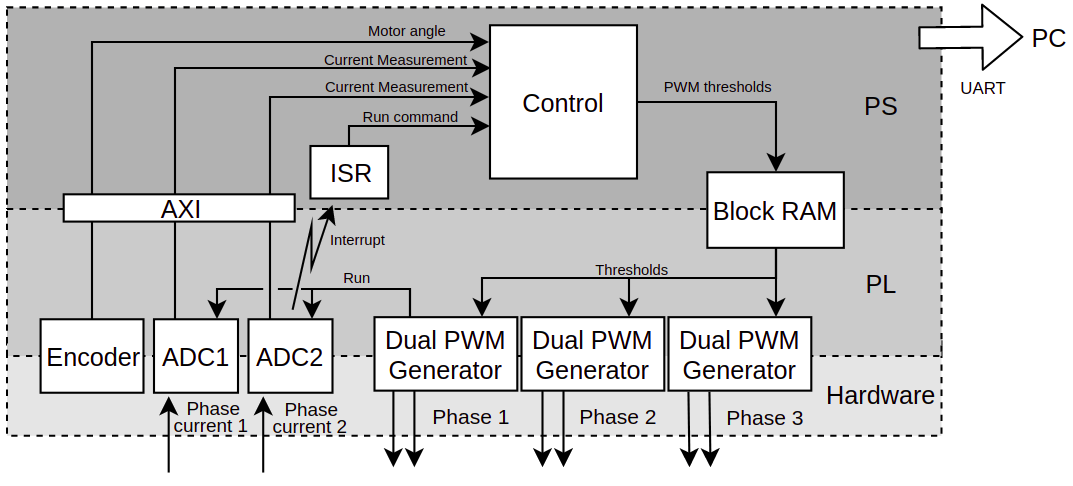
\includegraphics[width=1\linewidth]{pictures/software/embedded_overview.png}
	\caption{Embedded system overview}
	\label{fig:embedded_overview}
\end{figure}


In the programmable logic the drivers for three dual PWM generator are implemented. Each PWM generator control one phase in the inverter. The PWM generators all generate a pulse in the middle of their PWM periods. One of these are parsed to the ADC's and used to trigger a reading of the phase currents and the torque pedal. When the ADC's are done converting all inputs they produce an interrupt that triggers the ISR in the processing system.

The ADC readings as well as the encoder readings are parsed to the processing system through the AXI interface.



On figure \ref{fig:software_flow} the flowchart of the control loop implemented on the processing system can be seen. The system is waiting to receive the run command from the ISR which is triggered once every PWM period, see section \ref{sec:isr} for more about the ISR. 


\begin{figure}[H]
	\centering
	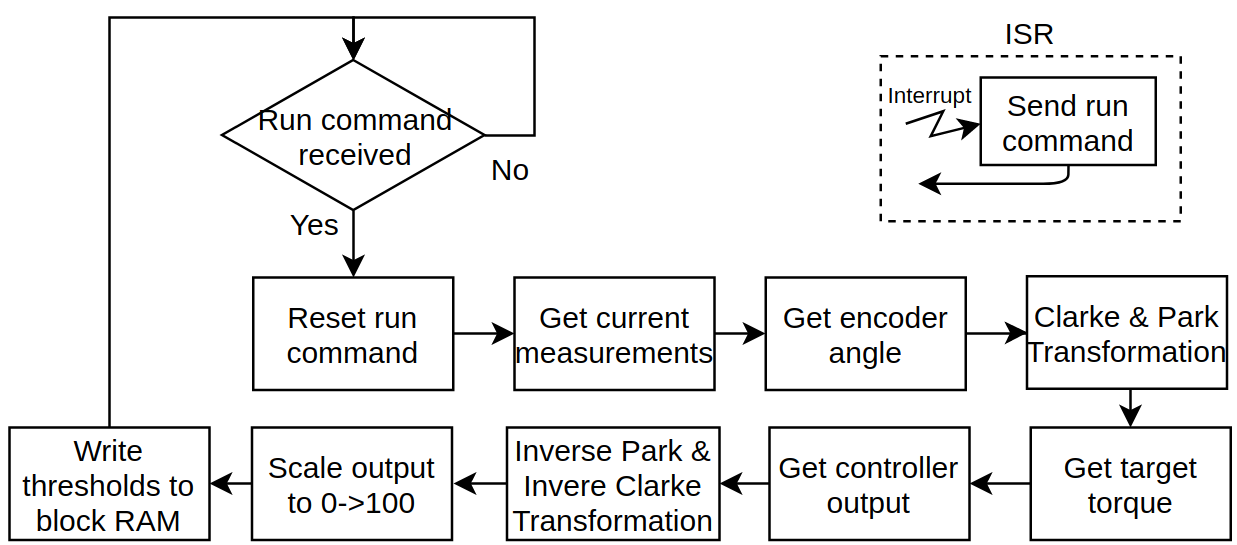
\includegraphics[width=0.9\linewidth]{pictures/software/software_flow.png}
	\caption{Processing System Overview}
	\label{fig:software_flow}
\end{figure}

When the run command is received it is first reset to get ready for the next command. Then the current measurements from the two ADC's are read into the system as well as the rotor angle from the encoder. A Clarke and a Park transformation is performed. The torque pedal position is read and the two PI controllers as discussed in section \ref{sec:control_system} perform the control. The result from the controllers are then transformed with an Inverse Park and an Inverse Clarke Transformation which produces three control signals. These signals are then linearly mapped to the range $0 \rightarrow 100$, which is what the PWM generators are compatible with. 
The thresholds are then written to a piece of block RAM shared between the PS and the PL. The PS will then wait for the next run command.





%%%%%%%%%%%%%%%%%%%%% PL %%%%%%%%%%%%%%%%%%%%%
\subsection{Programmable Logic (PL)}
% PWM generator
\subsubsection{PWM module}
\label{sec:pwm}
Each phase of the inverter is controlled by a PWM signal for the high-side and low-side of each leg.

The module shown on figure \ref{fig:pwm_module} is made to control a whole leg. Three instances of the module can be used to control all three phases.
\begin{figure}[H]
	\centering
	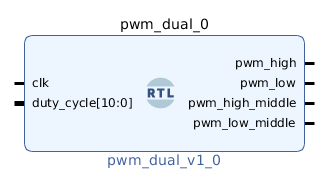
\includegraphics[width=0.5 \textwidth]{pictures/software/pwm_module.png}
	\caption{The PWM module made to control both high-side and low-side transistors of a leg in the inverter.}
	\label{fig:pwm_module}
\end{figure}
The module takes in a clock signal and a target duty cycle. The module then output two PWM signals inverse of each other and two pulse signals each sending out a pulse in the middle of their respective PWM signal.


\subsubsection*{Counter}
A counter is used for implementing the PWM. For every rising edge of the input clock the counter takes one step up or down depending on its current counting direction. When it reaches one of its outer limits the counting direction is switched as can be seen on figure \ref{fig:counter}.

\begin{figure}[H]
	\centering
	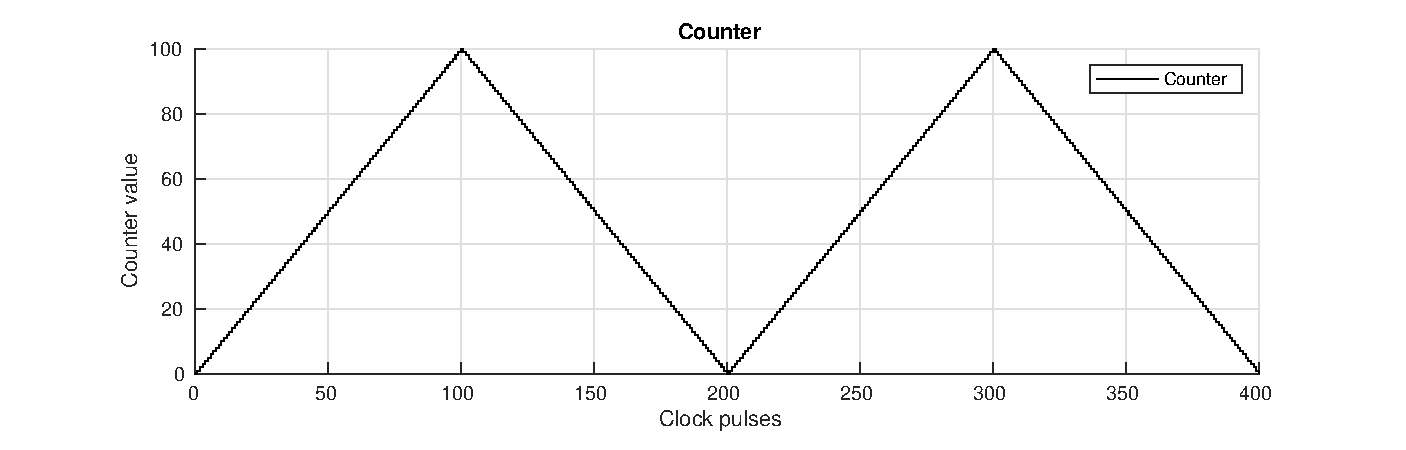
\includegraphics[width=1 \textwidth]{pictures/software/counter.eps}
	\caption{How the counter is counted up and down over time.}
	\label{fig:counter}
\end{figure}

The resolution of the PWM duty cycle is chosen to be $1\%$ which means the counter takes $100$ steps from minimum to maximum. The PWM is made as a phase correct PWM which means it will have the same phase no matter the duty cycle. Therefore the counter counts both up and down per period which results in $200$ steps per period. 

The signal out of the PWM generator should be the same frequency as the inverter components are designed for in the earlier sections which is $10kHz$. The input clock is already prescaling the output frequency by the number of counter steps but this is not enough and therefore in order for the PWM to have the correct frequency an additional prescaler is added. The prescaler value is found with equation \ref{eq:additional_prescaler}.

The prescaler is constructed with a counter counting up a value, $x$. When the value is reached the output clock is flipped and the counter is reset. Such a prescaler has a build in prescaling of 2 which is added besides the additional prescaler leading to equation \ref{eq:additional_prescaler1}.



\begin{subequations}
    \begin{align}
        \begin{split}
            f_{s} = \frac{f_{pl}}{c_{steps} \cdot x \cdot 2}
            \label{eq:additional_prescaler1}
        \end{split} \\ 
        \begin{split}
             x = \frac{f_{pl}}{f_{s} \cdot c_{steps} \cdot 2}
        \end{split} \\ 
        \begin{split}
            x = \frac{125MHz}{10kHz \cdot 200 \cdot 2} = 31.25 \sim 31
            \label{eq:additional_prescaler}
        \end{split} \\
        \begin{split}
            \frac{125MHz}{200 \cdot 31 \cdot 2} = 10.08kHz
        \end{split}
    \end{align}
\end{subequations}

Where $f_{s}$ is the output frequency of the PWM signal, $c_{steps}$ is the number of counter steps in a period, $f_{pl}$ is the logic clock which is $125MHz$ and $x$ is the additional prescaler.

With the additional prescaler the PWM module outputs PWM signals with a frequency of $10.08kHz$.

\subsubsection*{PWM}


To handle both a high-side PWM and low-side PWM each of the signals have a threshold and the output signal changes from high to low or opposite when the counter crosses the threshold as can be seen in figure \ref{fig:counter_with_pwm}. The two thresholds are spaced out with a static deadtime between them which is discussed later in this section. The deadtime on figure \ref{fig:counter_with_pwm} has been exaggerated to make it more visible.

\begin{figure}[H]
	\centering
	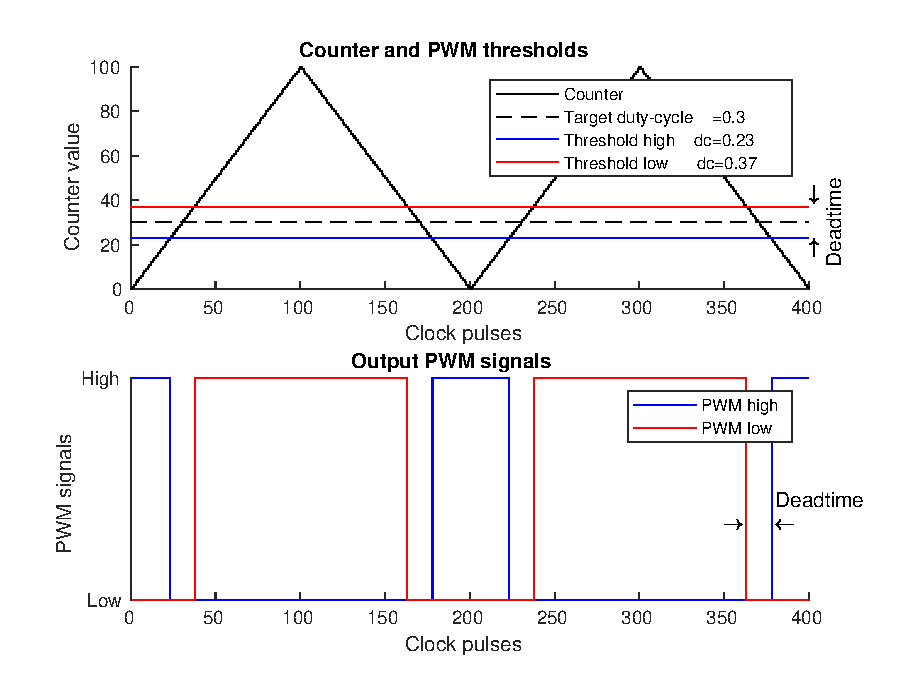
\includegraphics[width=0.85 \textwidth]{pictures/software/counter_with_pwm.eps}
	\caption{The top shows the target duty-cycle together with the thresholds compared to the PWM counter. The bottom shows the output PWM signals. The deadtime is exaggerated to make it more visible.}
	\label{fig:counter_with_pwm}
\end{figure}

The high-side PWM is high when the counter is below the high-side threshold, $counter < th_{high}$, otherwise it is low. 

The low-side PWM is high when the counter is above the low-side threshold, $counter > th_{low}$ otherwise it is low.

The VHDL code can be seen below.

\begin{minted}[frame=single,framesep=2mm,baselinestretch=1.2,linenos,fontsize=\footnotesize]{vhdl}
-- Control of the high side PWM
pwm_high <= HIGH when (counter < threshold_high) else LOW;
-- Control of the low side PWM
pwm_low  <= HIGH when (counter > threshold_low) else LOW;
\end{minted}
\begin{center}
    The VHDL code to control the PWM signals.
\end{center}


To avoid shorting the supply deadtime is inserted between turning off one transistor and turning on the other.

On figure \ref{fig:turn_off_time1} the conducted current for each transistor is drawn next to the PWM signals with deadtime being bigger than the transistor turn off time, $dead \ time > t_{turn \ off}$, which results in one transistor turning completely off before the other turns on. 

\begin{figure}[H]
	\centering
	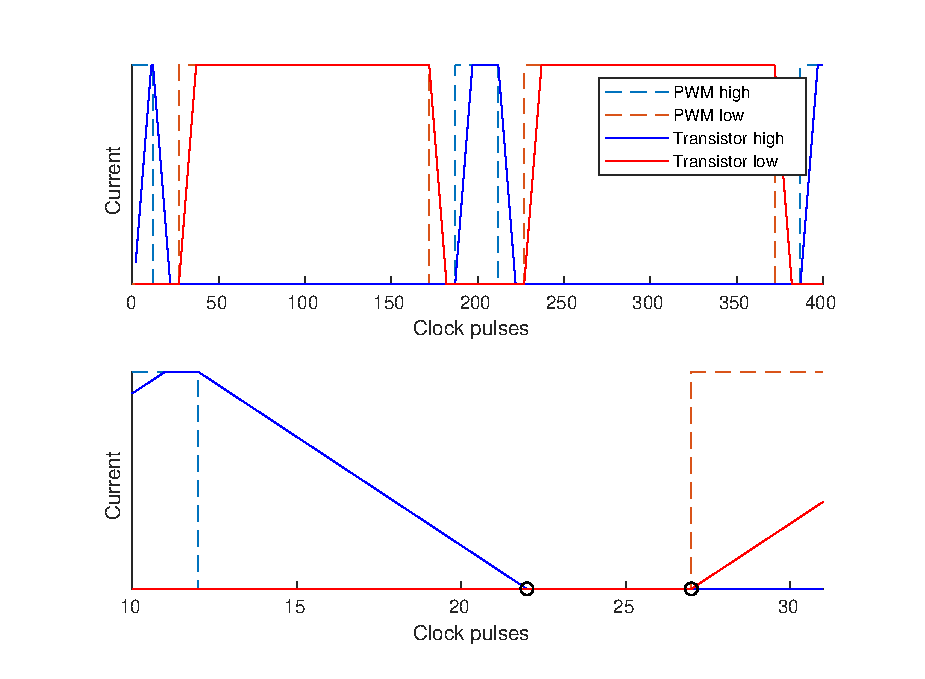
\includegraphics[width=0.8 \textwidth]{pictures/software/turn_off_time1.eps}
	\caption{PWM with deadtime and transistor conduction curves for systems with $dead \ time > t_{turn \ off}$}
	\label{fig:turn_off_time1}
\end{figure}

On figure \ref{fig:turn_off_time2} the conducted current for each transistor is drawn next to the PWM signals but this time the deadtime is smaller than the transistor turn off time, $dead \ time < t_{turn \ off}$, which results in both transistors conducting at the same time.
When both transistors conduct the supply is shorted which should be avoided especially when the supply consist of batteries.

\begin{figure}[H]
	\centering
	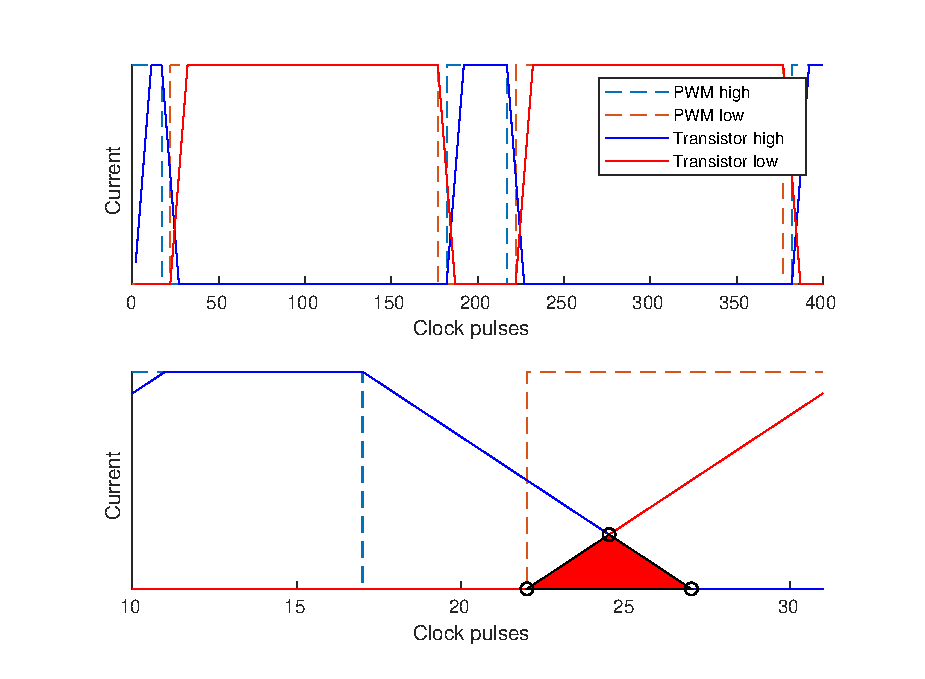
\includegraphics[width=0.8 \textwidth]{pictures/software/turn_off_time2.eps}
	\caption{PWM with deadtime and transistor conduction curves for systems with $dead \ time < t_{turn \ off}$}
	\label{fig:turn_off_time2}
\end{figure}

It is therefore important to choose the deadtime big enough to avoid shorting but also not so big that the systems performance is unnecessarily reduced.
\bigskip


To avoid compromising the required deadtime at edge cases where one of the thresholds tries to move above $100 \%$ or  below $0 \%$ the thresholds are found in two different ways.





When the high-side threshold is greater than the counter minimum plus half of the deadtime it is placed half of the deadtime below the threshold.
\begin{equation}
    th_{duty \ cycle} \geq  c_{min} + \frac{t_{dead \ time}}{2}
    \label{eq:threshold_high_condition}
\end{equation}
\begin{center}
    $\Downarrow$    
\end{center}
\begin{equation}
   th_{high} = th_{duty \ cycle} - \frac{t_{dead \ time}}{2}  
   \label{eq:threshold_high_equation}
\end{equation}

Otherwise the threshold is clamped to the counter bottom edge $th_{high} = counter_{min}$ which is possible because the PWM is switched when $th_{high} > counter$.
If the threshold comes too close to the edge the threshold will be clamped and the PWM will not switch. Had the PWM being switched when $th_{high} \geq counter$ this would not have worked.



The low-side threshold is placed half of the deadtime above the threshold when the duty cycle is at least half of the deadtime below the counter max.
\begin{equation}
    th_{duty \ cycle}\leq c_{max} - \frac{t_{dead \ time}}{2}
    \label{eq:threshold_low_condition}
\end{equation}
\begin{center}
    $\Downarrow$
\end{center}
\begin{equation}
  th_{low} = th_{duty \ cycle} + \frac{t_{dead \ time}}{2}  
  \label{eq:threshold_low_equation}
\end{equation}
Otherwise the threshold is clamped to the top counter edge.

The VHDL code to find the two thresholds can be seen below. The variable \textit{duty\textunderscore cycle} is parsed into the PWM module. \textit{DEADTIME}, \textit{HALF\textunderscore DEADTIME}, \textit{COUNT\textunderscore MIN} and \textit{COUNT\textunderscore MAX} are all constants.

\begin{minted}[frame=single,framesep=2mm,baselinestretch=1.2,linenos,fontsize=\footnotesize]{vhdl}
-- Get half of deadtime
HALF_DEADTIME(6 downto 0) <= DEADTIME(7 downto 1);
-- Find the threshold for the high-side PWM
threshold_high <= duty_cycle - HALF_DEADTIME when 
                (duty_cycle >= COUNT_MIN + HALF_DEADTIME) else COUNT_MIN;
-- Find the threshold for the low-side PWM
threshold_low  <= duty_cycle + HALF_DEADTIME when 
                (duty_cycle <= COUNT_MAX - HALF_DEADTIME) else COUNT_MAX;
\end{minted}
\begin{center}
    The VHDL code to find the thresholds for the high and low side PWM signals. The conditions and equations used are \ref{eq:threshold_high_condition}, \ref{eq:threshold_high_equation}, \ref{eq:threshold_low_condition} and \ref{eq:threshold_low_equation}.
\end{center}



The turn off times for the transistors was found in section \ref{sec:switching_power_loss} to be $75ns$.
The way deadtime is implemented it has to be defined as some even amount of ticks at the PWM frequency.
The minimum deadtime step, $dt_{res}$, in this system is calculated with equation \ref{eq:minimum_deadtime_resolution}.

\begin{subequations}
    \begin{align}
        \begin{split}
            dt_{res} = \frac{T}{2} \cdot \frac{dt_{min}}{c_{max}}
        \end{split} \\ 
        \begin{split}
             dt_{res} = \frac{2}{fs} \cdot \frac{dt_{min}}{c_{max}}
        \end{split} \\ 
        \begin{split}
             dt_{res} = \frac{2}{10kHz} \cdot \frac{2}{100} = 4\mu s
        \end{split} 
    \end{align}
    \label{eq:minimum_deadtime_resolution}
\end{subequations}

Which gives the system a safety margin of $\sim 53$ on the deadtime between the two PWM signals.


\subsubsection*{ADC Pulses}

To trigger a new reading by the ADC the PWM generator module has a build-in pulse mechanism that outputs a pulse in the middle of each of the PWM periods as can be seen on figure \ref{fig:adc_pulses}. Only the pulse in the middle of the high-side PWM is used to trigger the ADC. The reason for measuring in the middle of the PWM is to avoid majority of the ringing produced on the signals from switching.

\begin{figure}[H]
	\centering
	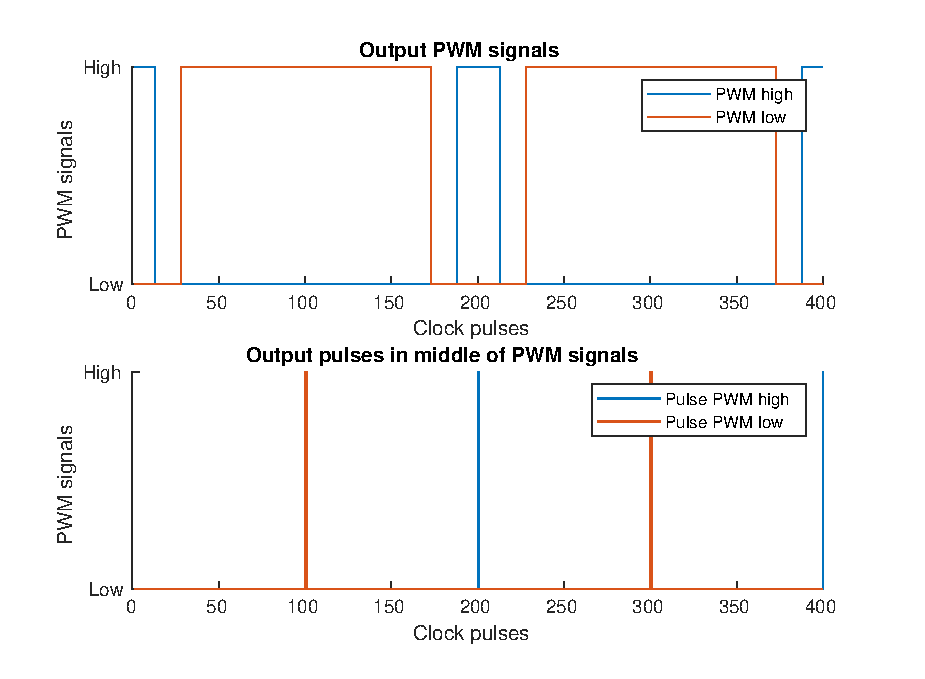
\includegraphics[width=0.8 \textwidth]{pictures/software/adc_pulses.eps}
	\caption{The top graph shows the high and low side PWM signals. The bottom graph shows the ADC pulses triggered in the middle of each PWM signal.}
	\label{fig:adc_pulses}
\end{figure}

The code for evaluating the signal states can be seen below. 
% The code utilizes the concurrent nature of VHDL which makes it fast and robust.
When the counter reaches its bottom edge the high pulse is set high and as soon as the counter starts going up again the signal is set low. The low pulse is controlled in the same way but this happens at the high counter edge instead.

\begin{minted}[frame=single,framesep=2mm,baselinestretch=1.2,linenos]{vhdl}
-- Output a pulse in the middle of the high PWM signal
pwm_high_middle <= HIGH when (counter <= COUNT_MIN) else LOW;

-- Output a pulse in the middle of the low PWM signal
pwm_low_middle <= HIGH when (counter >= COUNT_MAX) else LOW;
\end{minted}
\begin{center}
    The VHDL code to control the ADC pulses.
\end{center}


\subsubsection*{Test of PWM module}

To test the PWM generators a test scenario is set up. A simulated rotor angle and simulated currents are parsed into the control system and the outputs are measured with an oscilloscope. 
The maximum sine frequency expected out of the system is $333Hz$. To figure out how fast the simulated angle should change the time between each angle change is found. 
The angle is chosen to with $1$ degree steps. That gives a change rate of:


\begin{equation}
    change_{rate} = sin_{freq} \cdot 360^o
\end{equation}
Where $sin_{freq}$ is the target sine frequency. Which results in a time per angle of
\begin{equation}
    t_{angle} = \frac{1}{change_{rate}} = \frac{1}{333Hz \cdot 360^o} = 8 \mu s
\end{equation}
Where $t_{angle}$ is the time per angle. 

No currents will run in the system so the currents need to be simulate as well. The angle is used to calculate three sinusoidal curves. The way the three currents are calculated can be seen in equation \ref{eq:simulated_currents}.

\begin{equation}
    i_A = sin(angle), \ \ i_B = sin(angle + 120^o), \ \ i_C = sin(angle + 240^o)
    \label{eq:simulated_currents}
\end{equation}


Implementing this gives the PWM signal on one of the phases as seen in the top of figure \ref{fig:one_phase} and the resulting sine curve on the bottom.

\begin{figure}[H]
	\centering
	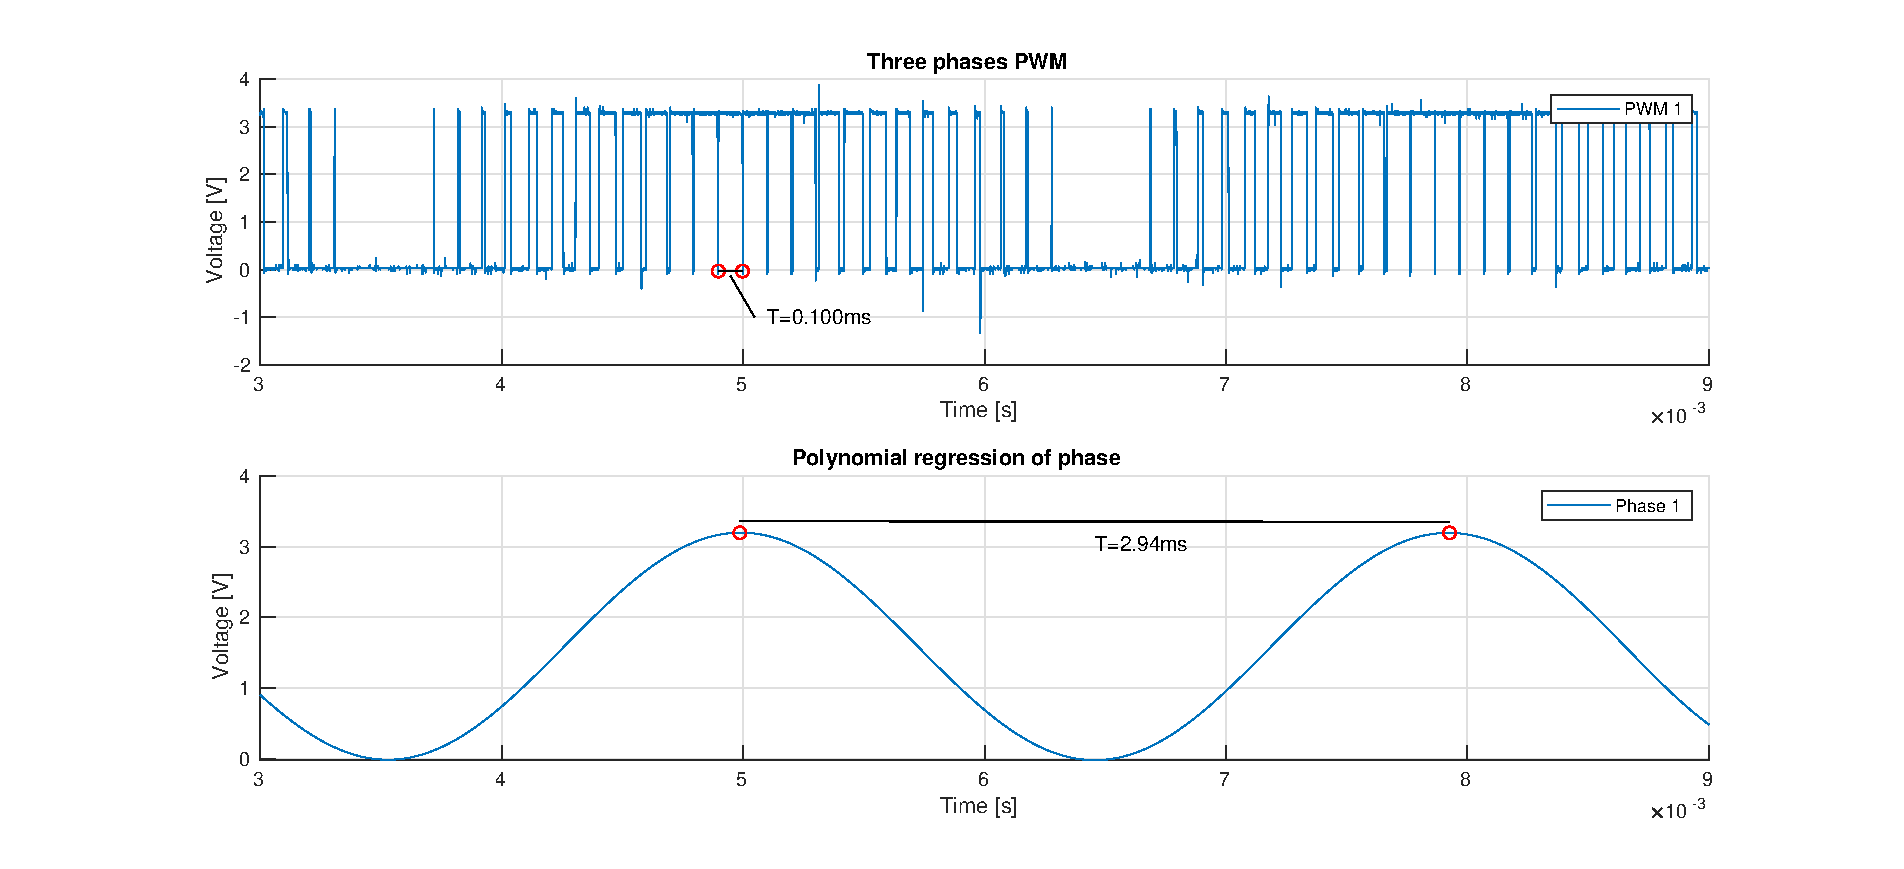
\includegraphics[width=1 \textwidth]{pictures/software/one_phase.eps}
	\caption{Testing of one phase. The top graph shows the PWM signals. The bottom graph shows the resulting sine curve found with a polynomial regression.}
	\label{fig:one_phase}
\end{figure}

The PWM frequency can be found by measuring the time between the middle of two PWM periods as can be seen in equation \ref{eq:pwm_frequency}. 
\begin{equation}
    f_s = \frac{1}{0.100 \cdot 10^{-3}} = 10kHz
    \label{eq:pwm_frequency}
\end{equation}
With a precision of 6 decimals on the time period the frequency of the PWM signal turns out to be $10kHz$.

The resulting sine can be found by applying a polynomial regression to the PWM signal which results in a sinusoidal curve. The frequency is found from the inverse of the time period between two points exactly one period apart. 
\begin{equation}
    sin_{freq} = \frac{1}{2.94 \cdot 10^{-3}} = 340 Hz
\end{equation}
The frequency of the sine is $340Hz$.

On figure \ref{fig:one_phase} only one of the phases are shown. In reality the system outputs three phases and all can be seen on figure \ref{fig:three_phases}. The periods in between the peak of the three phases are shown to determine the amount of phase shift. The time of one third of a period is calculated with \ref{eq:one_third_period}.
\begin{equation}
    \frac{1}{3} \cdot \frac{1}{340 Hz} = 0.9804ms
    \label{eq:one_third_period}
\end{equation}
By comparing the theoretical and measured periods between the phases it is determined that the phases are phase shifted with approximately $120^o = 2 \pi / 3 \ rad$.
\begin{figure}[H]
	\centering
	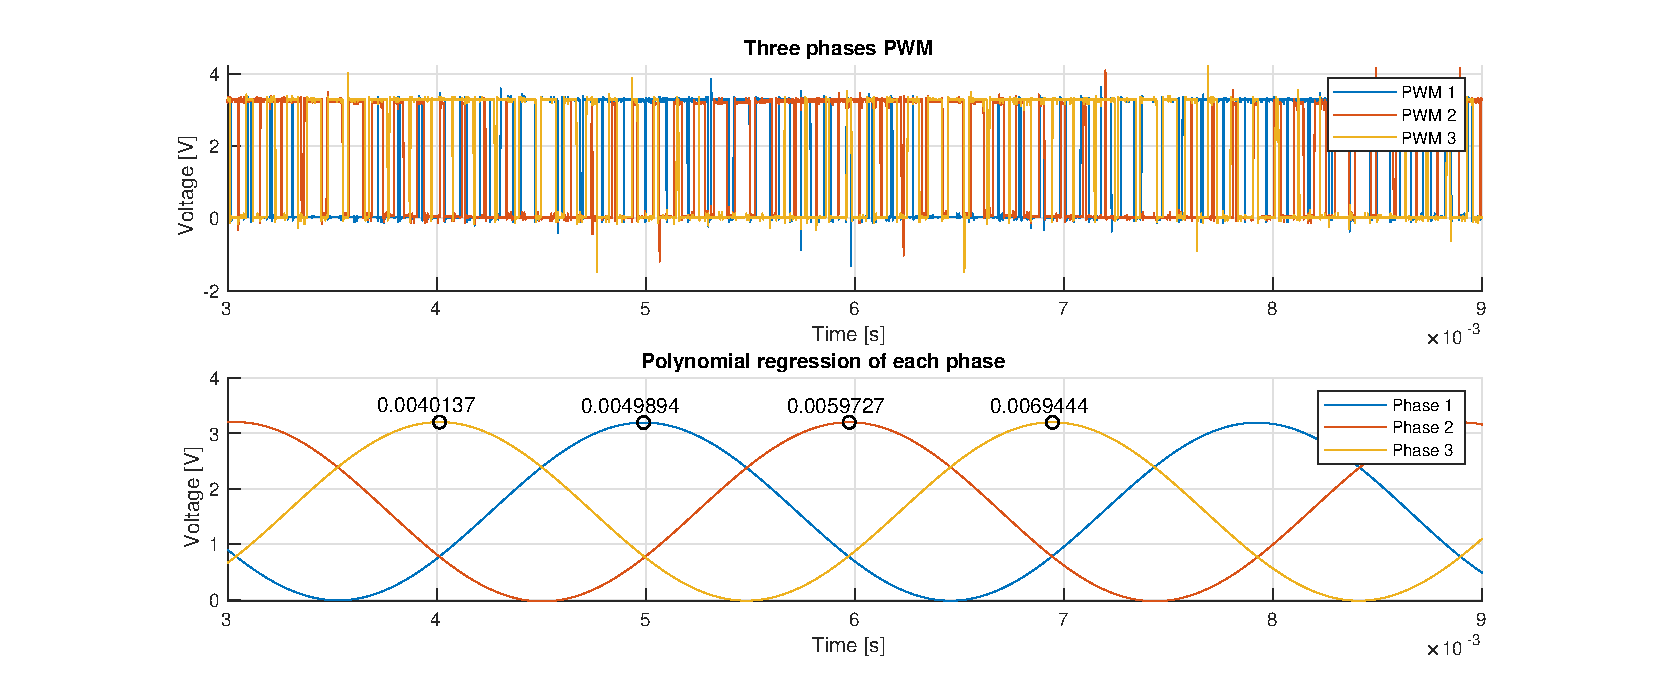
\includegraphics[width=1 \textwidth]{pictures/software/three_phases.eps}
	\caption{Testing of all three phases. The top graph shows the PWM signals. The bottom graph shows the resulting sine curves found with polynomial regressions.}
	\label{fig:three_phases}
\end{figure}


% Encoder
\subsubsection{Encoder}
\label{sec:encoder}

A driver module for the encoder on the motor was part of the material to get started on this project. \cite{encoder_module}

\begin{figure}[H]
	\centering
	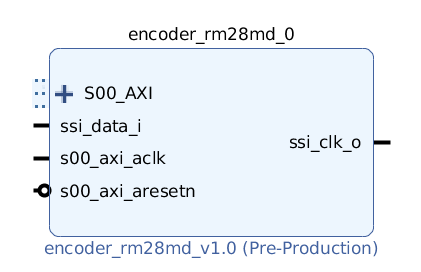
\includegraphics[width=0.4\textwidth]{pictures/software/encoder_module.png}
	\caption{The encoder driver module.}
	\label{fig:encoder_module}
\end{figure}
The driver module, as seen on figure \ref{fig:encoder_module}, supports an 8-bit encoder and takes care of handling the returned signal from the encoder itself. The module outputs the current rotor angle at a frequency determined by the PL clock and can be found with equation \ref{eq:encoder_frequency}.
\begin{equation}
f_{encoder} = \frac{f_{pl}}{6708} = \frac{125MHz}{6708} = 18.634kHz
\label{eq:encoder_frequency}
\end{equation}
The system runs at $10kHz$ which means the control loop will always have a new encoder angle at every cycle.


The encoder is a 8 bit encoder which means it has a resolution of $2^8 = 255$ steps per revolution. The motor has $4$ pole pairs which means the electric field inside the motor turns $4$ times each time the rotor turns $1$ time which means the resolution of the electric field angle is $1/4th$ of the mechanical rotor angle.
The two angles are both shown in figure \ref{fig:rotor_vs_electric_angle} where it can be seen that the electric angle moves 4 times faster than the rotor angle.

\begin{figure}[H]
	\centering
	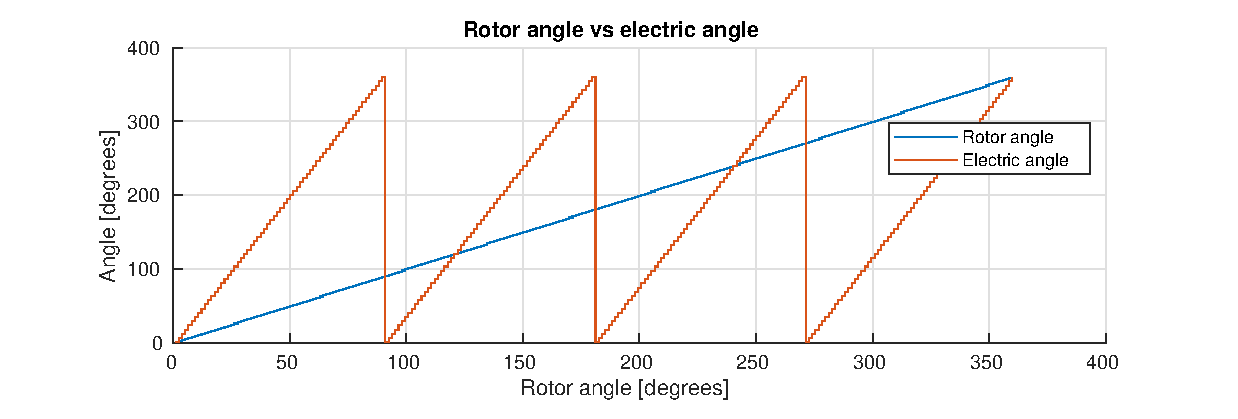
\includegraphics[width=1\textwidth]{pictures/software/rotor_vs_electric_angle.eps}
	\caption{Electric angle shown again the rotor angle.}
	\label{fig:rotor_vs_electric_angle}
\end{figure}

The resolution on the rotor angle and the electric angle can be calculated with equation \ref{eq:rotor_angle_error} and equation \ref{eq:electric_angle_error} respectfully. 

\begin{equation}
res_{rotor} = \frac{360^o}{2^8} = 1.412^o
\label{eq:rotor_angle_error}
\end{equation}

\begin{equation}
res_{electric} = \frac{360^o}{2^6} = 5.625^o
\label{eq:electric_angle_error}
\end{equation}




The rotor position is returned as an 8 bit value from the encoder module, and before the angle can be used in the control system it is first mapped from $0 \rightarrow 255$ to an actual angle going from $0^o \rightarrow 359^o$. The mapping is done with equation \ref{eq:angle_mapping}.
\begin{equation}
    angle = \frac{359}{255} \cdot position
    \label{eq:angle_mapping}
\end{equation}



\begin{lstlisting}[style=c, caption=Function to read an angle from the encoder. The angle is returned in degrees., label=code:encoder_angle_function]
f32 getRotorAngle(){
    u8 position = RM28MD_POSITION & 0x000000FF;     // Only the first byte is valid
    f32 angle   = 359/255 * position;       	      // Map position (0->255) to 
                                                    // angle (0->359)
    return angle;                                   // Return angle
}
\end{lstlisting}


\paragraph{Improve angle accuracy with linear interpolation}
\label{sec:linear_interpolation}
Low resolution and thereby big steps in the rotor angle results in uneven rotation of the motor especially at low speeds.
To improve the angle before it is used in the control the real angle is approximated with the use of linear interpolation. It is assumed that the rotor speed is approximately the same for each encoder value step. This assumption is not completely correct because it would mean the motor does not change speed. The rotor acceleration and deceleration is assumed slow enough compared to the encoder frequency to not result in big errors.


The formula for linear interpolation \cite{lin_interpol} can be seen in equation \ref{eq:linear_interpolation1}. 

\begin{equation}
    y = \Big( \frac{y_2-y_1}{x_2-x_1} \Big)(x-x_1)+y_1
    \label{eq:linear_interpolation1}
\end{equation}
Figure \ref{fig:angle_interpolation1} shows the scenario where the real angle, at point $p_2$, can be found from the measured angle, $p_1$, if $x_1$,$x_2$,$y_1$ and $y_2$ are known.
The equation can be converted to fit the system by setting the two $y$ values equal to the amount of change between the current and last step $\Delta a = y_2 - y_1$ and setting the $x$ values to be the step width $x_{step} = x_2 - x_1$. Assuming that the speed is approximately the same for the current step as it was on the last. Which results in equation \ref{eq:linear_interpolation2}.

\begin{equation}
    y =  \frac{\Delta a}{x_{step}} \Delta x+y_1
    \label{eq:linear_interpolation2}
\end{equation}

\begin{figure}[H]
	\centering
	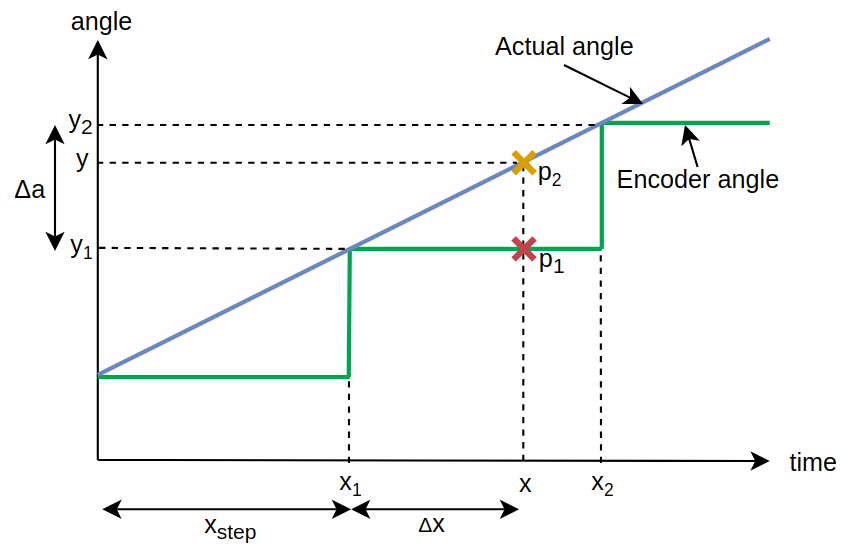
\includegraphics[width=0.8\textwidth]{pictures/software/angle_interpolation1.png}
	\caption{Ideal linear interpolation.}
	\label{fig:angle_interpolation1}
\end{figure}

The x-axis is discrete time and will be kept track of in relation to the number of samples passing and therefore $x$ will be denoted $n$. To know how fast the encoder values change over time this frequency is calculated with equation \ref{eq:encoder_step_frequency}.

\begin{equation}
    f = \frac{v_{[^o/s]}}{res_{rotor}} = 5000 [RPM] \cdot 6 \cdot \frac{360^o}{2^8} = 42188Hz
    \label{eq:encoder_step_frequency}
\end{equation}

The frequency is more than four times faster than the sampling frequency which means that not every encode value step will be sampled. The interpolation will only work if the is at least 2 samples on a step. To find the maximum speed where the interpolation works it is found where the encoder step frequency is lower than $10kHz$.

\begin{subequations}
	\begin{align}
    	\begin{split}
        	10kHz > v_{RPM}\cdot 6 \cdot res_{rotor}
    	\end{split} \\ 
    	\begin{split}
        	v_{RPM} < \frac{10kHz}{6 \cdot res_{rotor}}
    	\end{split} \\
    	\begin{split}
        	v_{RPM} < \frac{10kHz \cdot 2^8}{6 \cdot 360}
    	\end{split} \\
    	\begin{split}
        	v_{RPM} < 1185 RPM
    	\end{split} 
	\end{align}
\end{subequations}

When the rotor speed is less than $1185RPM$ the system will sample at least $1$ time per encoder step.

Equation \ref{eq:linear_interpolation2} can be further changed to fit the system.
\begin{equation}
    a_{i} = \frac{\Delta a}{n_{step}} n_{samples} + a
    \label{eq:linear_interpolation3}
\end{equation}
% Where $n_{step}$ is the number of samples on the last step and $n_{samples}$ is the amount of samples before the current sample on the same step as can be seen in figure \ref{fig:angle_interpolation2}.
Where $a_{i}$ is the interpolated angle, $n_{step}$ is the number of samples on the last step, $n_{samples}$ is the number of samples before the current sample on the current step, $a$ is the angle received from the encoder, as can be seen in figure \ref{fig:angle_interpolation2}.

\begin{figure}[H]
	\centering
	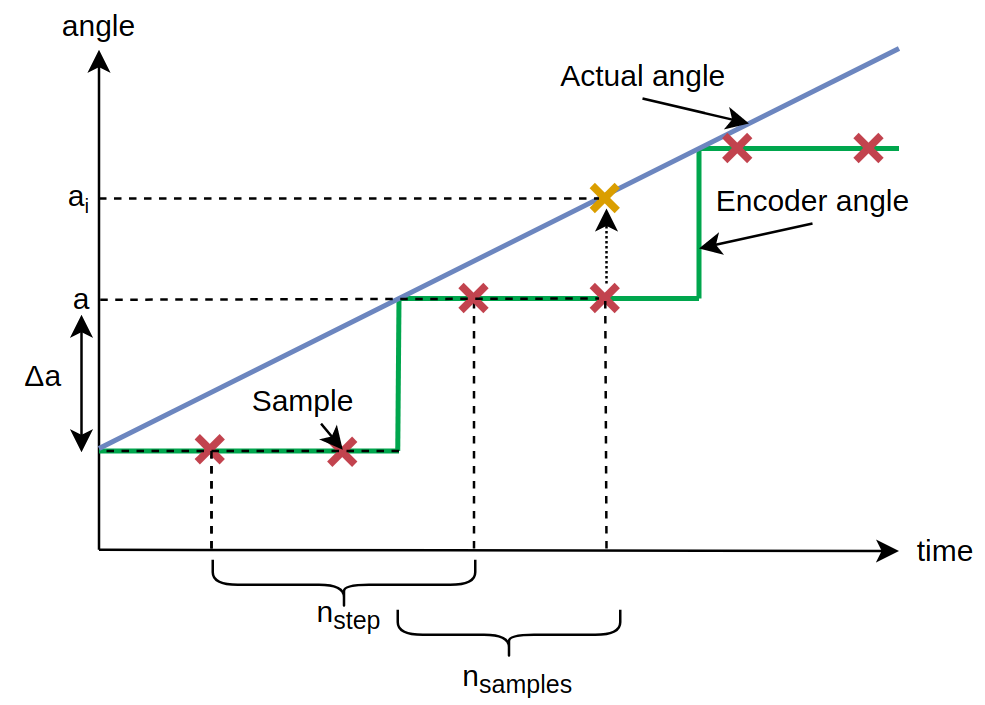
\includegraphics[width=0.8\textwidth]{pictures/software/angle_interpolation2.png}
	\caption{Practical version of linear interpolation.}
	\label{fig:angle_interpolation2}
\end{figure}






% The motor maximum speed is $5000RPM$ so the interpolation should be able to handle steps being skipped.

Equation \ref{eq:linear_interpolation3} can be rewritten to have the two counters as the fraction resulting in equation \ref{eq:linear_interpolation}.
\begin{equation}
a_{i} =  \frac{n_{samples}}{n_{step}} \Delta a  + a
\label{eq:linear_interpolation}
\end{equation}

$n_{samples}$ are a count of the number of samples on the current step. The counter starts at $0$ which means $n_{samples} \leq n_{steps}$ if the speed is approximately the same for the current and last encoder step.

\begin{equation}
	0 \leq	\Big(\frac{n_{samples}}{n_{step}} \Big) \leq 1
\end{equation}
Which means that the output of the interpolation is limited to
\begin{equation}
	 a \leq a_i \leq (a + \Delta a)
\end{equation}


The finished interpolation algorithm can be seen in the code snippet \ref{code:interpolation_algorithm} below. 

Every time the function is called a counter, \textit{time}, is incremented and this counter keeps track of the time.

Line $5$ to $8$ handle the first time the interpolation is used and it updates the variable $t\textunderscore 1$ which is the time of the left edge of the counter $n_{step}$. 

Line $10$ to $15$ handles the interpolation until the right edge of $n_{step}$ is updated, this is done with the variable $t\textunderscore 2$. For both the edges the value from the encoder is saved from the encoder to handle the step size in case one or more steps are skipped.

Line $17$ to $29$ handle the actual running algorithm. The sample counter is incremented. If a new step is reached the left edge is set the the last right edge, $t\textunderscore 1 = t\textunderscore 2$, and the new right edge is updated, $t\textunderscore 2 = angle$.

The step width is calculated as well as the step size which results in all the variable ready to calculate the interpolated angle on line $28$ as per equation \ref{eq:linear_interpolation}.

\begin{lstlisting}[style=c, caption=Interpolation algorithm implemented on the embedded system., label=code:interpolation_algorithm]
f32 interpolateAngle(f32 angle){
	time++;								                 // Keep track of time
	f32 angleInterpolated = angle;		     // Default value of angle
	/* First time used */
	if(t1 == 0){
		t1 = time;						               // Update time of t1
		t1v = angle;					               // Update angle of t1
	}
	/* If t2 has not been updated for the first time yet */
	if(t2 == 0){
		if(angle != t1v){				             // Check if first step happens
			t2 = time;					               // If so update time for t2
			t2v = angle;				               // Update angle of t2
		}
	}
	/* For all other steps than the first two */
	if(t1 != 0 && t2 != 0){				         // Do the actual interpolation
		nSamples++;						               // Keep track of samples on current step
		if(angle != t2v){				             // If new step happens
			t1 = t2;					                 // Move t2 to t1
			t1v = t2v;					               // Update value of t1
			t2 = time;					               // Update t2 to current time
			t2v = angle;				               // Update value of t2 to current angle
			nSamples = 0;				               // Reset number of samples on step
		}
 		u32 nStep = t2 - t1;				         // Get time on last step (approximation)
		f32 angleStep = t2v-t1v;	           // Get angle step
		angleInterpolated = nSamples/nStep * angleStep + angle; // Calculate new angle
	}
	return angleInterpolated;			         // Return new angle
}
\end{lstlisting}

To measure the improvement of the interpolated angle compared to the encoder angle a sweep of the motor speed from 1RPM to 5000RPM has been performed. The sweep was done with the algorithm implemented in Matlab. The results are shown on figure \ref{fig:interpolation_error}. The interpolated error is smaller for speeds less than $1185RPM$ otherwise the interpolation error is the same as the general error.


\begin{figure}[H]
	\centering
	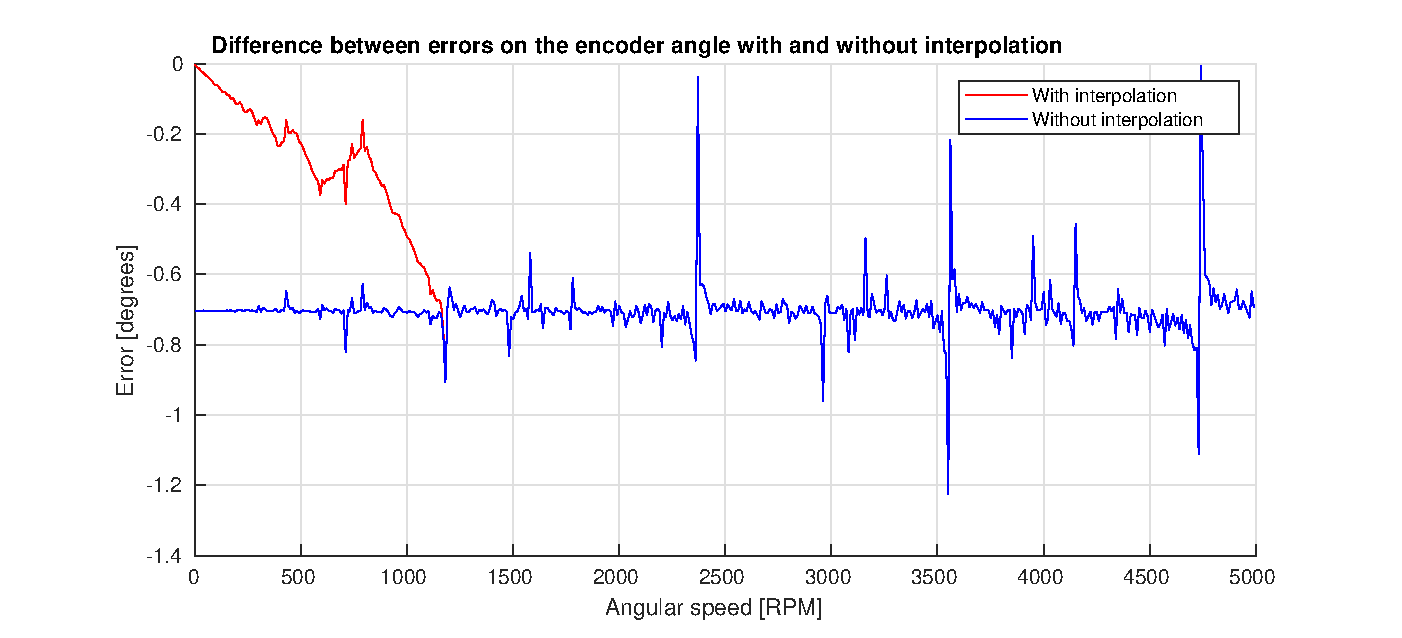
\includegraphics[width=1\textwidth]{pictures/software/interpolation_error.eps}
	\caption{Frequency sweep of angular error with and without linear interpolation.}
	\label{fig:interpolation_error}
\end{figure}


\subsubsection*{Conclusion}
The angle interpolation works to limit the encoder angle error for speeds under $1185RPM$ but speeds over $1185RPM$ the interpolation just follows the normal encoder angle error.

%ADC
\subsection{Analog-to-Digital Converter (ADC)}

To measure the phase currents once per PWM cycle and also the torque reference from the torque pedal an ADC is used. The Zynq has two 12 bit ADCs which enables it to sample two signals simultaneously. It is important to sample the phase current same time to avoid distortion by having a small time delay between current samples. 

Due to the symmetry between the three phases only two of the phases needs to be measured and the last can be caltulated with equation \ref{eq:third_phase}.
\begin{equation}
    I_C = -(I_A + I_B)
    \label{eq:third_phase}
\end{equation}
The calculation of the last phase is done in the processing system.

To control the ADC the IP block \textit{XADC} is used which can be seen on figure \ref{fig:adc_module}. 

\begin{figure}[H]
	\centering
	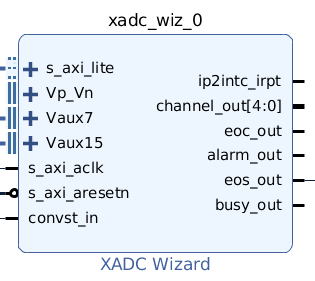
\includegraphics[width=0.35\textwidth]{pictures/software/adc.png}
	\caption{IP core to handle the two ADC in the Zynq.}
	\label{fig:adc_module}
\end{figure}

The block is configured to be triggered by an external signal which is connected to one of the ADC pulses produced by a PWM module.

While the phase currents are measured the torque pedal position is also measured. When all signals are measured the signal end-of-sequence, \textit{eos\textunderscore out}, outputs a pulse. The \textit{eos} signal is used to trigger the interrupt on the processing system as can be seen on figure \ref{fig:adc_block_diagram}.

\begin{figure}[H]
	\centering
	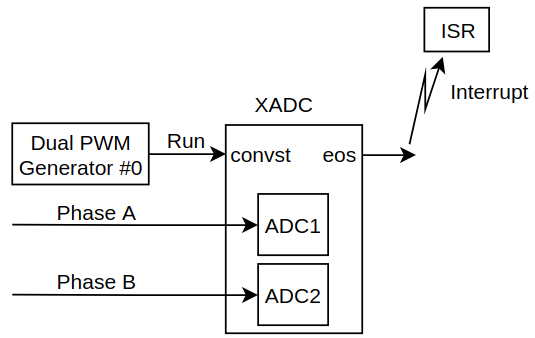
\includegraphics[width=0.5\textwidth]{pictures/software/adc_block_diagram.png}
	\caption{Function diagram showing the signals in and out of the ADC module.}
	\label{fig:adc_block_diagram}
\end{figure}





%%%%%%%%%%%%%%%%%%%%% PS %%%%%%%%%%%%%%%%%%%%%
\subsection{Processing System (PS)}
% Interrupt Service Routine ISR
\subsubsection{Interrupt Service Routine}
\label{sec:isr}
Every time an interrupt is triggered the ISR is called which sends a run command to the control loop to run. The interrupts are triggered with the same frequency as the PWM is running with, which is $10kHz$. Normal running behavior could look like the scenario shown on figure \ref{fig:isr1}. 

\begin{figure}[H]
	\centering
	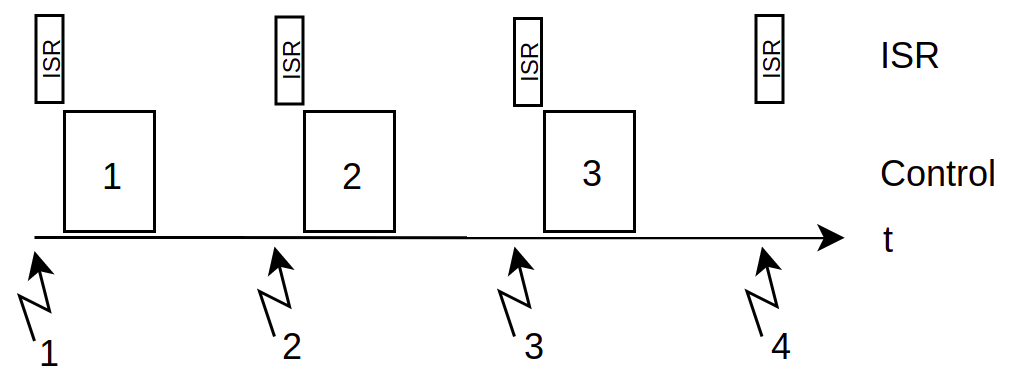
\includegraphics[width=0.65\linewidth]{pictures/software/isr/isr1.png}
	\caption{Normal running behavior of the interrupts coming in triggering the ISR which then triggers the control loop task.}
	\label{fig:isr1}
\end{figure}

Every time an interrupt is received the control loop is run and there is always some time between the control is run where the processor is idle.


The unlikely case where the control takes more time than the time between two interrupts can be seen in figure \ref{fig:isr2}. For robustness the system should be able to handle this situation. 

If the run command used by the ISR to trigger the control is a simple boolean variable set high by the ISR and reset as the first step in the control loop it is possible to get an interrupt while executing control. The running control will then finish and the new request will directly start executing.

\begin{figure}[H]
	\centering
	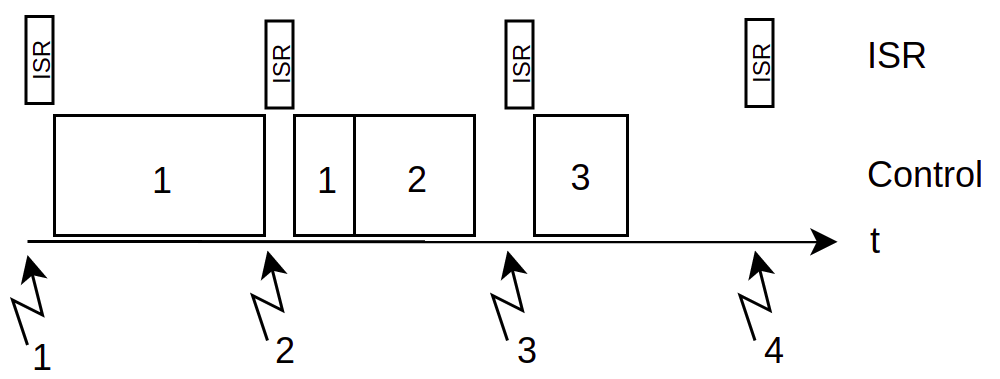
\includegraphics[width=0.65\linewidth]{pictures/software/isr/isr2.png}
	\caption{Unlikely scenario where a control task takes longer than the time between two interrupts.}
	\label{fig:isr2}
\end{figure}

Problems arise from this solution if the very unlikely event happen where multiple interrupts happen during the same control loop cycle as can be seen on figure \ref{fig:isr4}. Every interrupt before the last will be overlooked. In some systems overseeing an interrupt can be catastrophic but in this case it will improve the performance of the system compared to the alternative of executing all control tasks as can be seen on figure \ref{fig:isr3}.

\begin{figure}[H]
	\centering
	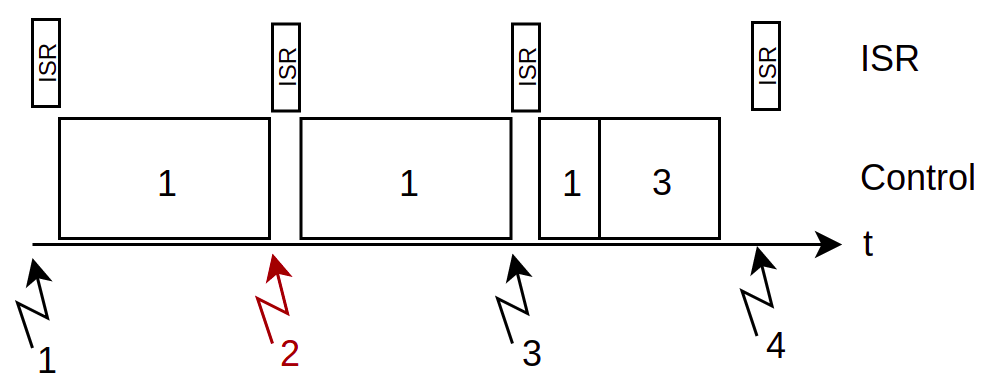
\includegraphics[width=0.65\linewidth]{pictures/software/isr/isr4.png}
	\caption{The scenario of a control task running for much longer than expected and skipping interrupts.}
	\label{fig:isr4}
\end{figure}

\begin{figure}[H]
	\centering
	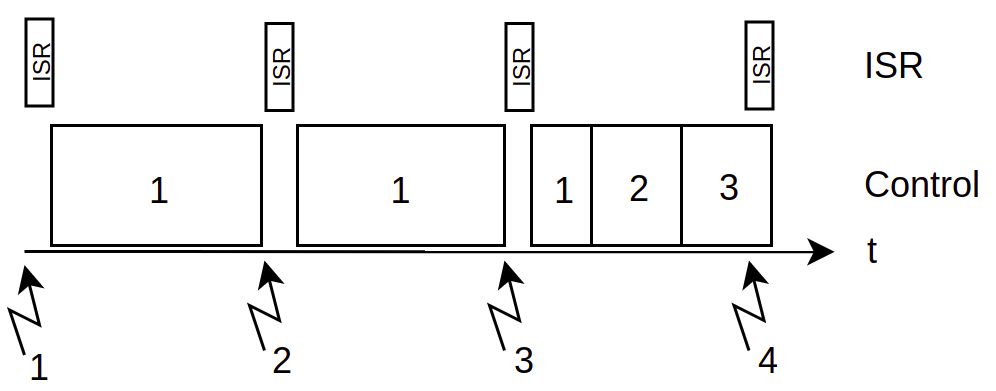
\includegraphics[width=0.65\linewidth]{pictures/software/isr/isr3.png}
	\caption{The scenerio of a control task running for much longer than expected but no interrupts are overseen.}
	\label{fig:isr3}
\end{figure}


Executing every control task will result in the system handling old data which is not relevant anymore. 

Therefore the run command used by the ISR to trigger the control loop is a simple boolean variable.

% Clarke Park
\subsubsection{Clarke Transformation and Park Transformation}
The control type chosen for the system is vector control also called field-oriented control and this requires Clarke/Park transformations as well as their inverse counterparts.
The transformations are implemented in the processing system and to limit the amount of calculations needed for each transformation all constants are defined beforehand.

% ******* Clarke Transformation ***********************************
\subsubsection*{Clarke Transform}


The embedded implementation of the Clark transformation as per equation \ref{eq:clarke_transformation} can be seen in code sample \ref{code:clarke}. The function creates two results and therefore instead of returning the values, the variables are declared outside the function calls and a pointer to the variables are parsed into the function.

\begin{lstlisting}[style=c, caption=Embedded Clarke Transformation., label=code:clarke]
/* The Clarke function */
void clarke(f32 *iAlpha, f32 *iBeta, f32 iA, f32 iB, f32 iC){
	*iAlpha = TWO_THIRDS * iA - ONE_THIRD * iB - ONE_THIRD * iC;
	*iBeta  = ONE_OVER_SQRT_THREE * iB - ONE_OVER_SQRT_THREE * iC;
}
\end{lstlisting}

% ************** Park Transformation ***********************************
\subsubsection*{Park Transform}
The embedded implementation of the Park transformation as per equation \ref{eq:park_transformation} can be seen in code sample \ref{code:park}. The transformation involves calculating the sine and cosine of the angle. These two functions are implemented by using look-up tables and are discussed in section \ref{sec:sine_cosine}.

\begin{lstlisting}[style=c, caption=Embedded Park Transformation., label=code:park]
/* The Park function */
void park(f32 *iD, f32 *iQ, f32 iAlpha, f32 iBeta, f32 angle){
	const f32 cosAngle = fastCos(angle);
	const f32 sinAngle = fastSin(angle);
	*iD = cosAngle * iAlpha + sinAngle * iBeta;
	*iQ = -sinAngle * iAlpha + cosAngle * iBeta;
}
\end{lstlisting}

The inverse Clarke and inverse Park transformations can be found in appendix \ref{app:inverse_park} and \ref{app:inverse_clarke}.


\paragraph{Sine and Cosine}
\label{sec:sine_cosine}
The trigonometric functions sine and cosine are implemented with a look-up table to improve performance. The sine function looks up a given angle in the table to find the output of the function. The cosine uses the sine function but offset the angle by $90 ^{\circ}$. 

To limit the amount of memory used only one value is saved per degree which results in $360$ saved values of type \textit{f32} which is based on the type \textit{float}. The variables are $4$ bytes resulting in $1440 bytes \sim 1.5kB$ used.
The maximum error that can exist because of the quantization is the biggest step between two values in the data set. 
The largest error is where the sine/cosine has the largest slope, and this is where it crosses 0 on the y-axis. The error is positive when the slope is positive and negative when the slope is negative. The maximum error is $\pm 1.75 \%$ as can be seen on figure \ref{fig:sinus_lookup_error}. 
\begin{figure}[H]
	\centering
	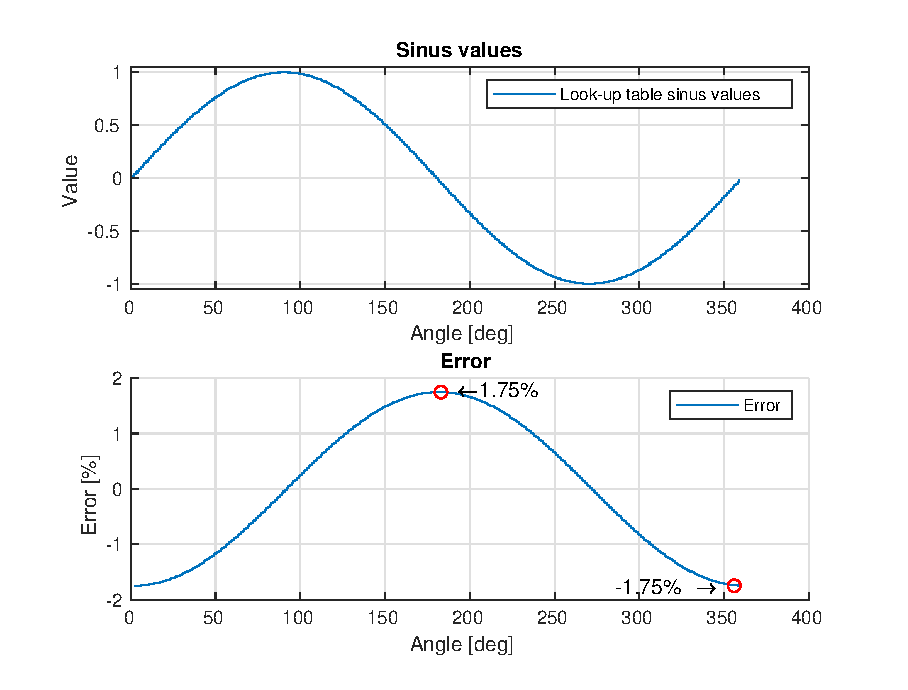
\includegraphics[width=0.6 \textwidth]{pictures/software/sinus_lookup_error.eps}
	\caption{Error between the real sine value and the look-up table value.}
	\label{fig:sinus_lookup_error}
\end{figure}



\begin{lstlisting}[style=c, caption=Sine and cosine implemented with look-up tables., label=code:lookup_table]
/* Sine lookup table */
#define SIN_N 		360	 // Number of data points in the sine constant array
const f32 sineValues[] = {0,0.0174524064372835,0.0348994967025010,...};

/* Function that returns sin(angle) */
f32 fastSin(f32 angle){
	unsigned int index = (unsigned int)angle;       // Truncate decimals
	return (f32)sineValues[index % SIN_N];      // 
}	

/* Function that returns cos(angle) */
f32 fastCos(f32 angle){
	f32 newAngle = (f32)((int)(angle + 90) % (int)360);
	return (f32)fastSin(newAngle);
}
\end{lstlisting}

% Controller
\subsubsection{Controller}
\label{sec:embedded_control}
The PI-controller is implemented in \textit{c} on the processing system in a object orientated way where each of the two controllers are defined together with their gains. When the system is booted up the controllers are initialized with the values and prepared for usage. The code for this can be seen in code sample \ref{code:pi_controller1}.

\begin{lstlisting}[style=c, caption=Initialization of PI-controller., label=code:pi_controller1]
/* Declare controllers */
Controller cQ, cD;
static f32 kpQ = 1, kiQ = 1, kpD = 1, kiD = 1;

void initControllers(){
    /* Initialize controllers with gains */
    initController(&cQ, kpQ, kiQ);
    initController(&cD, kpD, kiD);
}
\end{lstlisting}

When the motor is running the only thing needed to be done is to input the reference value and the current measured value to the controller and get a new output as can be seen in code sample \ref{code:pi_controller2}. The function 'getOutput()' handles the controller gains, keeping track of the integrator part and integrator windup.

\begin{lstlisting}[style=c, caption=Usage of PI-controller., label=code:pi_controller2]
    /* Run controller */
	f32 outD = getOutput(&cD, 0, iD);
	f32 outQ = getOutput(&cQ, getTargetTorque(), iQ);
\end{lstlisting}

The implementation of the 'getOutput()' function can be seen in code sample \ref{code:pi_controller3}.
First the controller gains \textit{kp} and \textit{ki} are retrieved. Then the controller's integrator part is updated and then retrieved.

The output of the controller is found with the following equation.
\begin{equation}
    u = k_p \cdot e + k_i \cdot int
\end{equation}

Where $u$ is the output, $e$ is the error which is the target minus the input, 

$e = target - input$, $int$ is the integrator part and $k_p$ and $k_i$ are the controller gains.

The integral part of the controller might experience integrator windup because the control execution is much faster than the motor acceleration. To handle this a simple output limitation is implemented to limit the controller output.



\begin{lstlisting}[style=c, caption=Implementation of PI-controller 'get output'-function., label=code:pi_controller3]
/* Function to get the next output of a controller with a new input */
f32 getOutput(Controller *c, f32 target, f32 input){
	f32 error = target - input;                         // Calculate error
	
	// Collect controller data
	const f32 kp  = getKp(c);
	const f32 ki  = getKi(c);
	addToIntegrator(c, error);
	const f32 integrator = getIntegrator(c);

	f32 output =  (kp * error) + (ki * integrator);     // Calculate new output
	
	// Anti integrator windup. Limit the output to within set limits
	if(output > MAX_OUTPUT){                            // Check upper limit
		output = MAX_OUTPUT;                              // Limit output
	}
	if(output < MIN_OUTPUT){                            // Check lower limit
		output = MIN_OUTPUT;                              // Limit output
	}	
	return output;                                      // Return new output
}
\end{lstlisting}



% Communication between PL and PS
\subsection{Communication between PL and PS}
Sending thresholds from the processing system to the PWM low-level modules are done through a piece of block RAM.
The build-in block RAM of the Zybo consist of a 36kbit storage area with two independent access ports. 

The PWM modules expect 8 bit thresholds which results in 24 bits or 3 bytes being used of the block RAM. 

A mere 3 bytes account for around $0.08\%$ of the total block RAM. While this is a waste of the block RAM, it was chosen because of it being easily accessible from both the PS and PL and easy to set up. 

When the control task on the processing system has run and produced the thresholds for each phase they are written into the first 3 bytes of the block RAM as can be seen on figure \ref{fig:com_pl_to_ps}.

\begin{figure}[H]
	\centering
	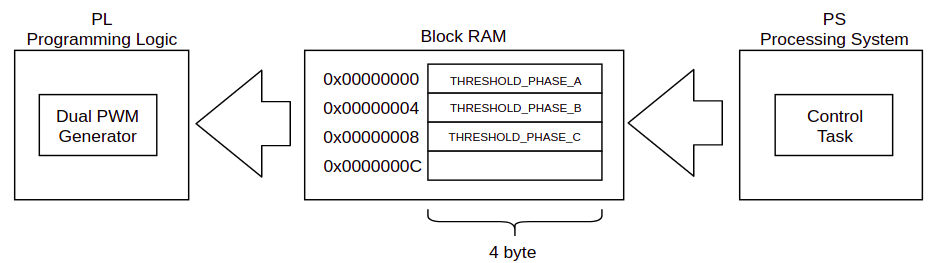
\includegraphics[width=1\linewidth]{pictures/software/com_pl_to_ps.png}
	\caption{Communication from PS to PL through block RAM.}
	\label{fig:com_pl_to_ps}
\end{figure}

From here the memory interface module in the logic can collect the thresholds and parse them unto the three PWM modules as can be seen on figure \ref{fig:com_pl}. The PWM modules then use the thresholds to produce the PWM signals as discussed in section \ref{sec:pwm}.


\begin{figure}[H]
	\centering
	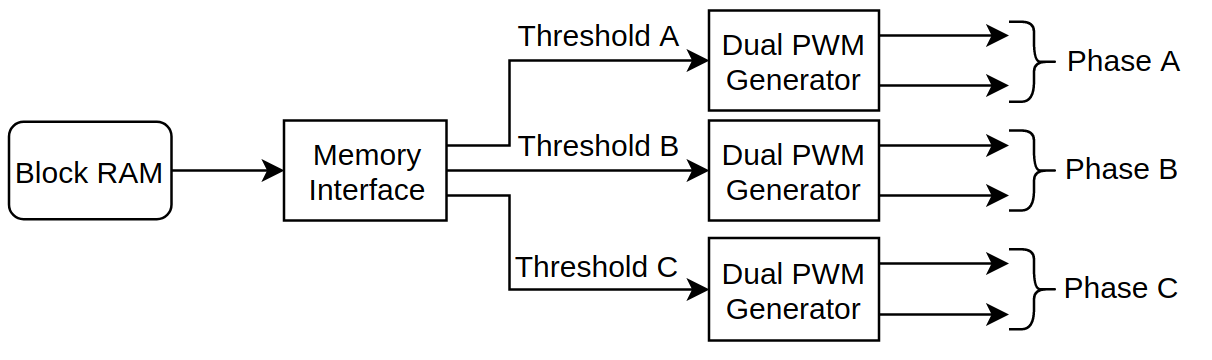
\includegraphics[width=0.8\linewidth]{pictures/software/com_pl.png}
	\caption{The data flow in the PL from the block RAM to the PWM generators.}
	\label{fig:com_pl}
\end{figure}




% Computer inteface
\subsection{Computer interface}

To keep track of the system, start the converter and change the gains for the controllers an interface between the embedded controller and a computer is made. The interface is made in a simple low-level way with a predefined message structure and limited error handling. The structure can be seen in table \ref{tab:message_structure}. 


\begin{table}[H]
\centering
\begin{tabular}{|l|c|c|c|c|c|c|}
\hline
\# character       & 1       & 2                 & 3            & 4            & 5       & 6   \\ \hline
Function      & ID  & Read / Write                     & \multicolumn{4}{c|}{Value}               \\ \hline
Valid Values & $0\rightarrow 9$ & 'r'/'w'  & \multicolumn{4}{c|}{$0\rightarrow 9999$} \\ \hline
\end{tabular}
\caption{Structure of the interface messages from the computer to the embedded controller.}
\label{tab:message_structure}
\end{table}

The first character of the message contains an ID of the variable that the message is referring to. The IDs of all variables included can be seen in table \ref{tab:variable_ids}.

The second character describes if the message is a read or write command.

The third till sixth character are only used for the write command. They contain the value to which the variable from the second character should be changed to. The format of the value can be seen in table \ref{tab:variable_ids}. To be able to handle digits the gains send as values from $0000 \rightarrow 9999$ but in the controller these are mapped to $00.00 \rightarrow 99.99$.


\begin{table}[H]
\centering
\begin{tabular}{|l|llll|} \hline
ID & Valid values                                               & Valid commands & Variable    & Unit       \\   \hline
0  & \begin{tabular}[c]{@{}l@{}}0 = Stop\\1 = Run \end{tabular} & 'r'/'w'        & Inverter state & - \\ \hline
1  & -                                                          & 'r'            & Speed       & Hz \\ \hline
2  & $0 \rightarrow 9999$                                                     & 'r'/'w'        & Ki\_D       & \begin{tabular}[c]{@{}l@{}}$1/100$ \\ \textit{Example: 1234 = 12.34}\end{tabular} \\ \hline
3  & $0 \rightarrow 9999$                                                     & 'r'/'w'        & Kp\_D       & \begin{tabular}[c]{@{}l@{}}$1/100$ \\ \textit{Example: 1234 = 12.34}\end{tabular} \\ \hline
4  & $0 \rightarrow 9999$                                                     & 'r'/'w'        & Ki\_Q       & \begin{tabular}[c]{@{}l@{}}$1/100$\\ \textit{Example: 1234 = 12.34}\end{tabular}  \\ \hline
5  & $0 \rightarrow 9999$                                                     & 'r'/'w'        & Kp\_Q       & \begin{tabular}[c]{@{}l@{}}$1/100$\\ \textit{Example: 1234 = 12.34}\end{tabular}  \\ \hline
\end{tabular}
\caption{List of variables that can be accessed through the communication between a computer and the embedded controller.}
\label{tab:variable_ids}
\end{table}

An example of how the communication can be seen on figure \ref{fig:pc_interface}. 

Line 1 is a command to write the value $03.46$ to \textit{Ki\textunderscore D}. 

Line 2 is a read command of the same variable. 

Line 3 is the reply from the embedded system.

Line 5 is a write command to start the inverter. Line 6 and 7 are the same as 2 and 3 but for the inverter state.

Line 9 is a command to write the value $15.23$ to the gain \textit{Ki\textunderscore Q}.

\begin{figure}[H]
	\centering
	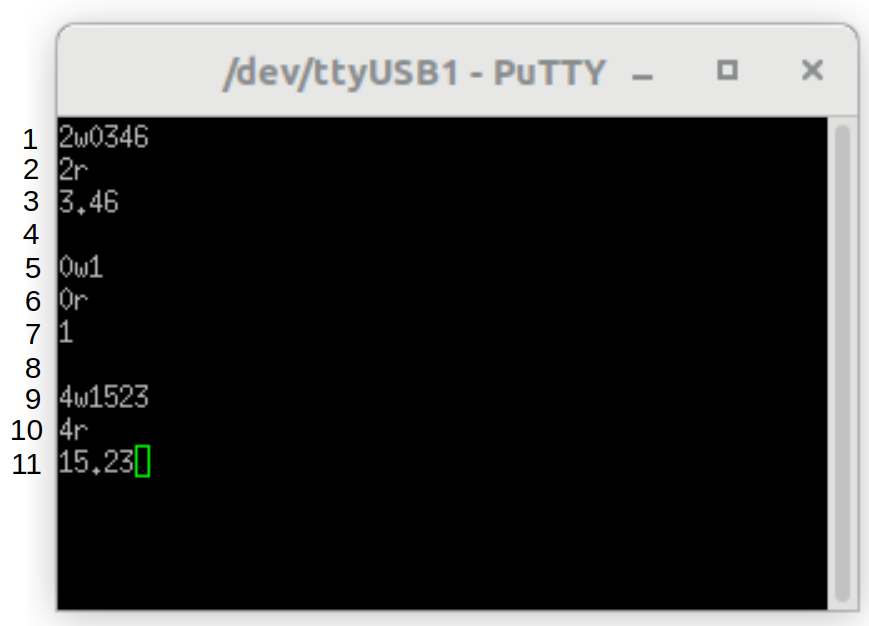
\includegraphics[width=0.65\linewidth]{pictures/software/pc_interface_terminal.png}
	\caption{Example of the computer interface used for communication between the embedded controller and a computer.}
	\label{fig:pc_interface}
\end{figure}



